\section{Learning-Based Tactile Manipulation}
\label{sec:learning}

This section surveys three paradigms for learning manipulation with tactile feedback---imitation learning, reinforcement learning, and force-informed approaches---along with optimization-based alternatives that compete with learned policies on structured tasks. Table~\ref{tab:learning} provides a comparative overview.

\begin{figure}[t]
\centering
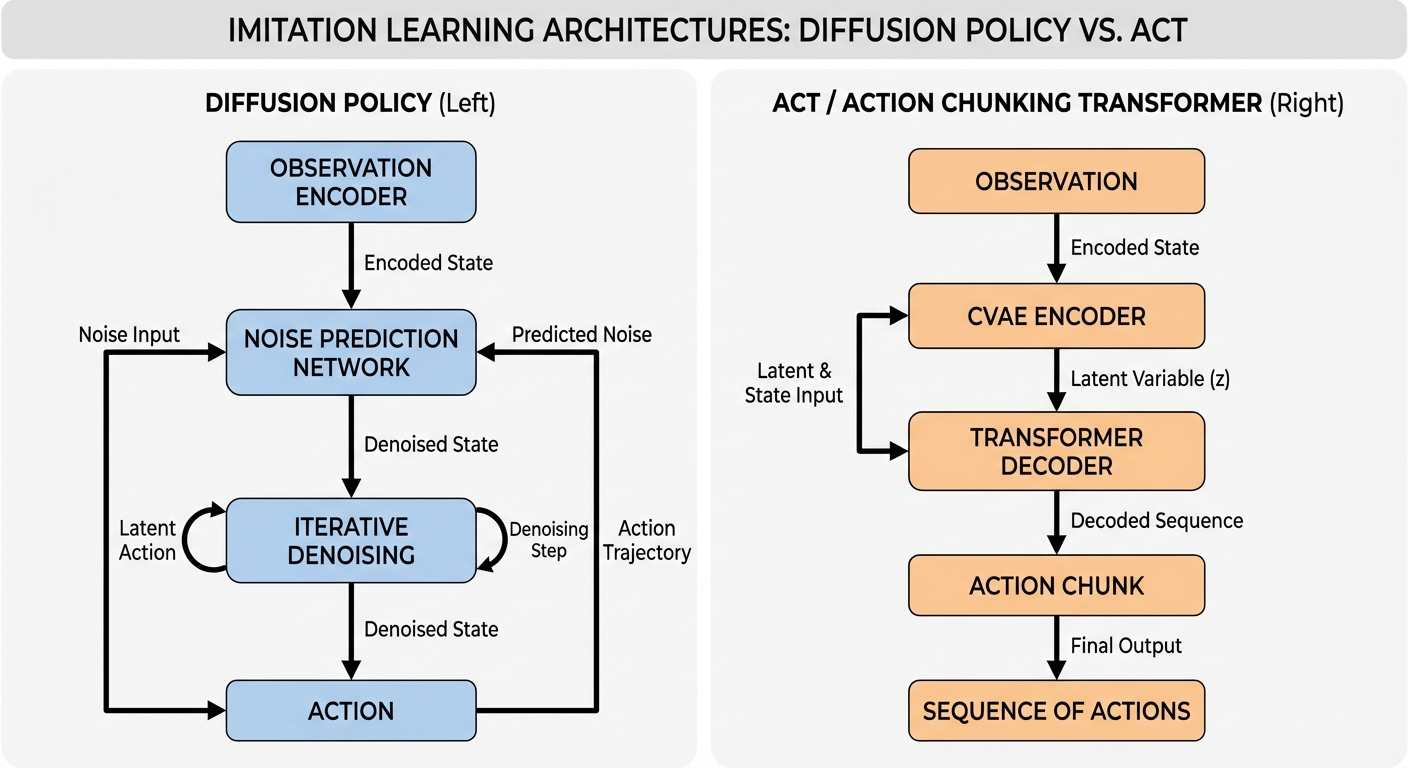
\includegraphics[width=\columnwidth]{../assets/figures/ch07/fig_7_1_diffusion_vs_act_academic.png}
\caption{Comparison of the two dominant imitation learning architectures for tactile manipulation: Diffusion Policy (conditional denoising process) and ACT/ALOHA (action chunking with Transformers). Both handle multimodal action distributions but differ in generation mechanism and temporal structure.}
\label{fig:il_architectures}
\end{figure}

\subsection{Imitation Learning}

Imitation learning (IL) trains policies by directly mimicking human demonstrations. Two architectures have dominated since 2023, both leveraging the expressivity of generative models to handle the multimodal action distributions characteristic of contact-rich manipulation.

\textbf{Diffusion Policy}~\cite{chi2023diffusion} (Columbia/MIT/TRI, RSS 2023, 500+ citations) models the robot's visuomotor policy as a conditional denoising diffusion process. Starting from Gaussian noise, iterative denoising produces action sequences conditioned on the current observation. This formulation naturally handles multimodal action distributions---a critical requirement when multiple valid manipulation strategies exist for the same observation---achieving 46.9\% average improvement over prior deterministic and VAE-based methods. The architecture's compatibility with tactile conditioning has made it the preferred backbone for contact-rich tasks: FARM~\cite{helmut2025farm} conditions Diffusion Policy on GelSight Mini tactile images for force-aware manipulation, while PP-Tac~\cite{lin2025pptac} integrates slip detection with diffusion-based control for thin-object grasping.

\textbf{ACT/ALOHA}~\cite{zhao2023aloha} (Stanford, RSS 2023, 400+ citations) takes a different approach via Action Chunking with Transformers (ACT), predicting sequences of future actions rather than single-step outputs. The key insight is that temporal chunking reduces the compounding error problem in sequential decision-making. On the sub-\$20K ALOHA bimanual hardware, ACT achieves 80--90\% success on fine-grained bimanual tasks from just 10-minute demonstrations---a data efficiency that makes the approach practical for rapid prototyping. Mobile ALOHA~\cite{fu2024mobilealoha} (200+ citations) extends the platform to mobile bimanual manipulation, representing one of the most influential end-to-end research systems.

\begin{figure}[t]
\centering
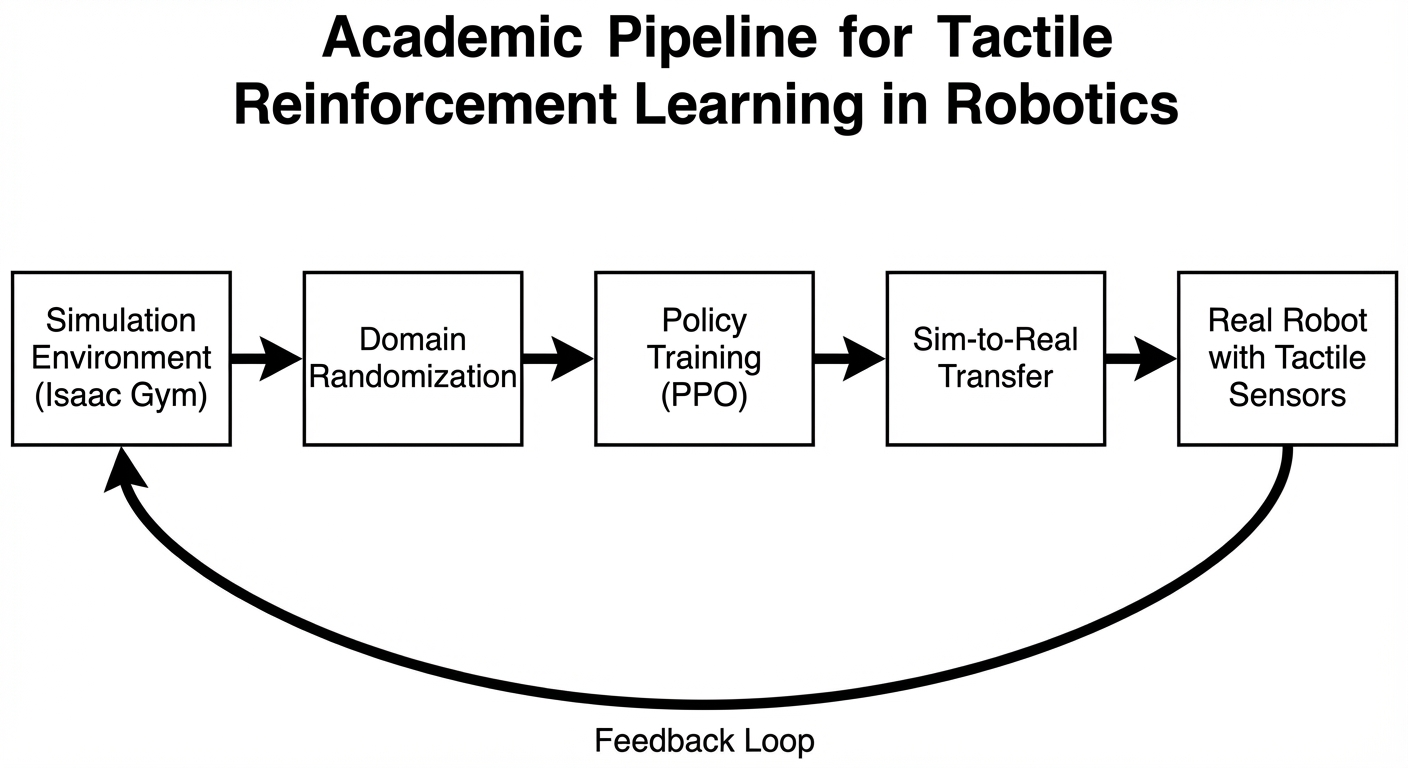
\includegraphics[width=\columnwidth]{../assets/figures/ch07/fig_7_2_tactile_rl_pipeline_academic.png}
\caption{Tactile reinforcement learning pipeline: policies are trained in simulation with domain randomization (physics and tactile parameters) and transferred zero-shot to real hardware. Binary tactile skin models with wide coverage have proven surprisingly effective for sim-to-real transfer.}
\label{fig:tactile_rl_pipeline}
\end{figure}

\subsection{Reinforcement Learning}

Reinforcement learning (RL) discovers manipulation policies through trial-and-error optimization of a reward signal, typically in simulation with subsequent transfer to physical hardware.

\textbf{OpenAI Dactyl}~\cite{openai2020dactyl} (\emph{IJRR}, 2020, 1{,}500+ citations) was the landmark demonstration that sim-to-real RL can solve contact-rich dexterous manipulation. Using a Shadow Hand in simulation with massive domain randomization, Dactyl learned to manipulate a Rubik's Cube and transferred zero-shot to the physical robot. The work established domain randomization as the primary strategy for overcoming the sim-to-real gap.

\textbf{DeXtreme}~\cite{handa2023dextreme} (NVIDIA, ICRA 2023, 200+ citations) advanced the state of the art with Automatic Domain Randomization (ADR) on Allegro Hand in Isaac Gym. ADR simultaneously randomizes both physics parameters (friction, mass, joint stiffness, gravity) and non-physics parameters (lighting, camera position, texture, background), with the randomization ranges automatically adjusted based on training progress. Combined with Omniverse Replicator for synthetic visual data, vision-based policies outperformed all prior literature on dexterous manipulation benchmarks.

\textbf{Tactile RL} has demonstrated that simplified sensor models with wide coverage can be surprisingly effective. Yin et al.~\cite{yin2023rotating} (RSS 2023) achieved continuous in-hand rotation using only binary tactile sensors---contact yes/no plus 3-axis direction---without any vision. The subsequent work~\cite{yin2024tactile} developed a binary 3-axis tactile skin simulation model running at 5{,}000~FPS, enabling zero-shot sim-to-real transfer with 93\% success on out-of-distribution objects. This result challenges the assumption that high-resolution sensors are always better: \emph{coverage of the entire hand surface may matter more than resolution at any single point}.

Human-in-the-loop RL~\cite{luo2025hil} (\emph{Science Robotics}, 2025) combines human intuition with autonomous policy optimization, achieving near-perfect success rates on precise assembly tasks within 1--2.5 hours of real-world training, outperforming pure RL baselines by 2$\times$.

\subsection{Tactile-Based Manipulation Methods}

\begin{table*}[t]
\caption{Comparison of Learning Methods for Tactile Manipulation}
\label{tab:learning}
\centering
\begin{tabular}{@{}L{2.8cm}cL{2.8cm}L{2.5cm}c@{}}
\toprule
\textbf{Method} & \textbf{Year} & \textbf{Approach} & \textbf{Tactile Input} & \textbf{Key Result} \\
\midrule
Yin et al.~\cite{yin2023rotating} & 2023 & RL, binary tactile & Binary 3-axis skin & 93\% OOD \\
Wu et al.~\cite{wu2025canonical} & 2025 & IL, canonical 3D & 3-axis tactile & 78\% avg \\
PP-Tac~\cite{lin2025pptac} & 2025 & Diffusion + slip & R-Tac sensor & 87.5\% thin \\
DexForce~\cite{chen2025dexforce} & 2025 & IL, spring model & 6-axis F/T & 76\% avg \\
ForceVLA~\cite{yu2025forcevla} & 2025 & VLA + MoE & 6-axis F/T & +23.2pp \\
FARM~\cite{helmut2025farm} & 2026 & Diffusion + tactile & GelSight Mini & Force-aware \\
TLA~\cite{hao2025tla} & 2025 & Language + tactile & 24K pairs & 85+\% \\
RGMC~\cite{yu2025rgmc} & 2025 & Optimization & Kinematic only & 5mm error \\
\bottomrule
\end{tabular}
\end{table*}

Several recent works demonstrate tactile feedback as increasingly critical for specific manipulation capabilities:

\textbf{PP-Tac}~\cite{lin2025pptac} (RSS 2025) addresses the extremely challenging problem of grasping thin objects---paper, cards, gaskets---where standard grippers fail completely. The system integrates an R-Tac round camera-based gel sensor, a lightweight CNN for real-time slip detection, an online force controller, and Diffusion Policy into a unified pipeline, achieving 87.5\% success on thin and deformable objects. This result demonstrates tactile's direct practical value on problems that vision alone cannot solve.

\textbf{TLA}~\cite{hao2025tla} (Tactile-Language-Action model) processes sequential tactile feedback via cross-modal language grounding, enabling natural language commands for contact-rich manipulation. With 24{,}000 tactile-action instruction pairs customized for fingertip peg-in-hole assembly, TLA achieves 85+\% success on unseen clearances and peg shapes, significantly outperforming standard diffusion policy baselines.

\subsection{Force-Informed Learning}

Two approaches explicitly integrate force information as a first-class modality:

\textbf{DexForce}~\cite{chen2025dexforce} (\emph{IEEE RA-L}) addresses the force information gap in teleoperation-collected demonstrations. Using a spring model $x_f = x_o + k_f \cdot f$ with a single parameter $k_f = 0.0045$, kinesthetic teaching naturally records force-torque information that teleoperation misses. Policies trained on force-informed actions achieve 76\% average success across 6 contact-rich tasks, while policies trained without force information achieve near-zero success---a dramatic demonstration that force is essential, not optional, for these tasks.

\textbf{ForceVLA}~\cite{yu2025forcevla} (NeurIPS 2025) introduces FVLMoE, a 4-expert Mixture-of-Experts architecture that dynamically routes force, vision, and language inputs based on task demands within a pi0-based VLA framework. The result is +23.2 percentage points over force-free baselines and 90\% success under visual occlusion---conditions where vision-only policies fail catastrophically. ForceVLA represents the direction of integrating tactile/force as a ``first-class modality'' in foundation models for manipulation.

\subsection{Optimization-Based Alternatives}

Not all manipulation requires learning. The RGMC Champion solution~\cite{yu2025rgmc} (\emph{IEEE RA-L}, ICRA 2025 competition winner and Most Elegant Solution) achieved 5~mm average error in large-range precise in-hand manipulation via pure kinematic trajectory optimization---without any pretraining, demonstration data, or simulation. This result establishes an important baseline: for well-structured problems with known kinematics, classical optimization can match or exceed learning-based approaches while providing interpretability and formal guarantees that learned policies cannot offer.
